\subsubsection{Analog Input GPIO (ADC)}
\label{sec:CubeMXADC}

Zur Spannungsmessung am Akkumulator ist der GPIO Pin \texttt{PB1} als Analog Input konfiguriert.
Dieser wird mit dem internen Analog zu Digitalwandler ADC1 auf dem Channel 9 ausgewertet.
Die Einstellungen hierfür sind in Abbildung \ref{pic:CubeMX_ADC} ersichtlich und entsprechen den Standardeinstellungen. Die Auflösung beträgt 12 Bit.

\begin{figure}[H]
	\centering
	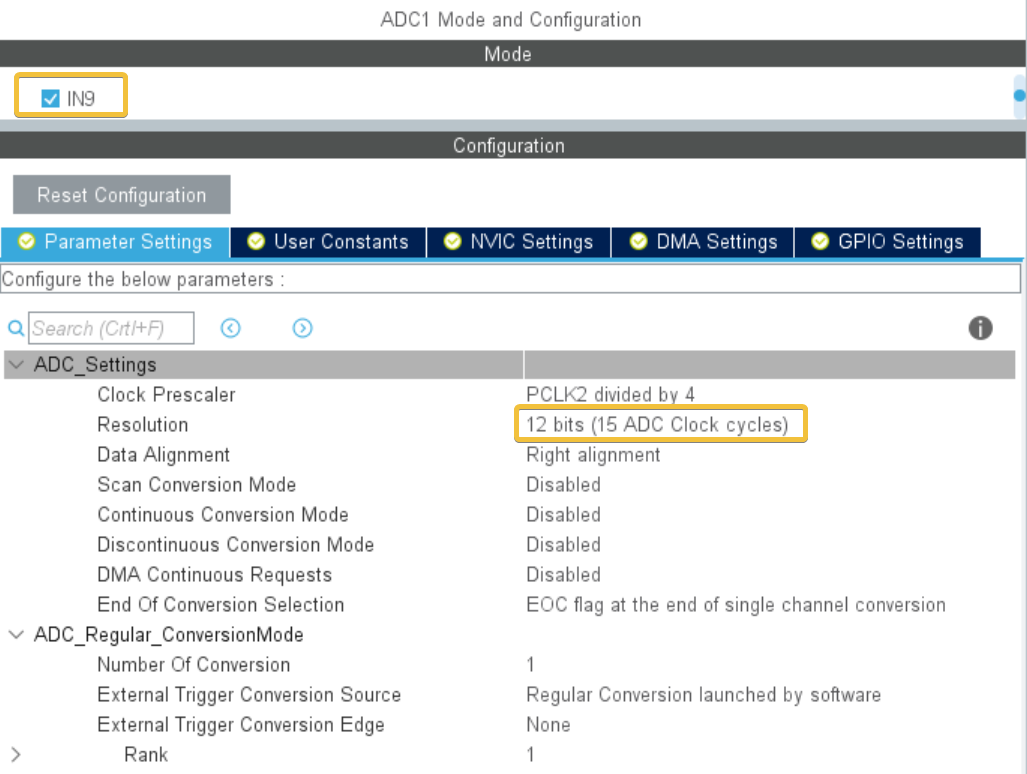
\includegraphics[width=0.9\linewidth]{CubeMX_ADC}
	\caption{Parameter Einstellungen ADC Wandlers 1}
	\label{pic:CubeMX_ADC}
\end{figure}


